\documentclass{ctexbeamer}
\usepackage{tikz}
\usepackage{minted} % 用于代码高亮
\usetheme{Madrid} % 选择beamer主题

\begin{document}

\title{TikZ 绘图示例}
\date{\today}

\frame{\titlepage}

\section{基本绘图}

\begin{frame}[fragile]
\frametitle{基本图形绘制}

\begin{block}{画点和连线}
下面是画一个点和一个连接的三角形的例子:
\begin{minted}[frame=single,framesep=10pt]{latex}
\documentclass{article}
\usepackage{tikz}
\begin{document}
\begin{tikzpicture}
    % 绘制点
    \fill (0,0) circle (2pt); % 画一个点,坐标为(0,0)
    % 绘制三角形
    \draw (0,0) -- (4,0) -- (2,3.5) -- cycle; % 画一个三角形
    % 标注点坐标
    \node at (0,0) [below left] {A(0,0)};
\end{tikzpicture}
\end{document}
\end{minted}

结果是一个简单的点和三角形:
\begin{tikzpicture}
    % 绘制点
    \fill (0,0) circle (2pt); % 画一个点,坐标为(0,0)
    % 绘制三角形
    \draw (0,0) -- (4,0) -- (2,3.5) -- cycle; % 画一个三角形
    % 标注点坐标
    \node at (0,0) [below left] {A(0,0)};
\end{tikzpicture}
\end{block}
\end{frame}

\begin{frame}[fragile]
\frametitle{长方形绘制}

\begin{block}{画长方形}
下面是绘制长方形的代码:
\begin{minted}[frame=single,framesep=10pt]{latex}
\documentclass{article}
\usepackage{tikz}
\begin{document}
\begin{tikzpicture}
    % 绘制长方形
    \draw (0,0) rectangle (4,3); % 左下角(0,0) 右上角(4,3)
    % 标注长方形的坐标
    \node at (0,0) [below left] {A(0,0)};
    \node at (4,0) [below right] {B(4,0)};
    \node at (4,3) [above right] {C(4,3)};
    \node at (0,3) [above left] {D(0,3)};
\end{tikzpicture}
\end{minted}

结果是一个长方形,带有顶点标注:
\begin{tikzpicture}
    % 绘制长方形
    \draw (0,0) rectangle (4,3); % 左下角(0,0) 右上角(4,3)
    % 标注长方形的坐标
    \node at (0,0) [below left] {A(0,0)};
    \node at (4,0) [below right] {B(4,0)};
    \node at (4,3) [above right] {C(4,3)};
    \node at (0,3) [above left] {D(0,3)};
\end{tikzpicture}
\end{block}
\end{frame}

\section{圆形和椭圆}

\begin{frame}[fragile]
\frametitle{圆形与椭圆绘制}

\begin{block}{画圆和椭圆}
下面是绘制圆和椭圆的代码:
\begin{minted}[frame=single,framesep=10pt]{latex}
\documentclass{article}
\usepackage{tikz}
\begin{document}
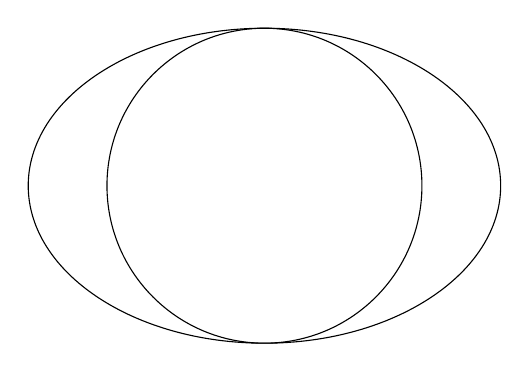
\begin{tikzpicture}
    % 绘制圆
    \draw (0,0) circle (2cm); % 圆心在(0,0),半径为2cm
    % 绘制椭圆
    \draw (0,0) ellipse (3cm and 2cm); % 圆心在(0,0),水平半径为3cm,垂直半径为2cm
\end{tikzpicture}
\end{minted}

结果是一个圆和一个椭圆:
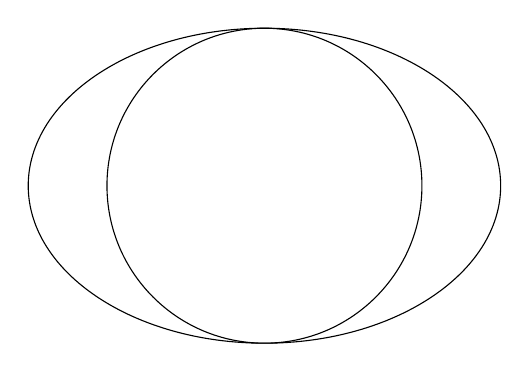
\begin{tikzpicture}
    % 绘制圆
    \draw (0,0) circle (2cm); % 圆心在(0,0),半径为2cm
    % 绘制椭圆
    \draw (0,0) ellipse (3cm and 2cm); % 圆心在(0,0),水平半径为3cm,垂直半径为2cm
\end{tikzpicture}
\end{block}
\end{frame}

\begin{frame}[fragile]
\frametitle{画圆弧}

\begin{block}{画圆弧}
下面是绘制圆弧的代码:
\begin{minted}[frame=single,framesep=10pt]{latex}
\documentclass{article}
\usepackage{tikz}
\begin{document}
\begin{tikzpicture}
    % 绘制圆弧
    \draw (0,0) arc[start angle=0, end angle=90, radius=2cm]; % 从0度到90度,半径2cm
\end{tikzpicture}
\end{minted}

结果是一个圆弧:
\begin{tikzpicture}
    % 绘制圆弧
    \draw (0,0) arc[start angle=0, end angle=90, radius=2cm]; % 从0度到90度,半径2cm
\end{tikzpicture}
\end{block}
\end{frame}

\begin{frame}[fragile]
\frametitle{标注圆心与顶点}

\begin{block}{标注圆心与顶点}
下面是一个示例,展示如何标注圆心和顶点:
\begin{minted}[frame=single,framesep=10pt]{latex}
\documentclass{article}
\usepackage{tikz}
\begin{document}
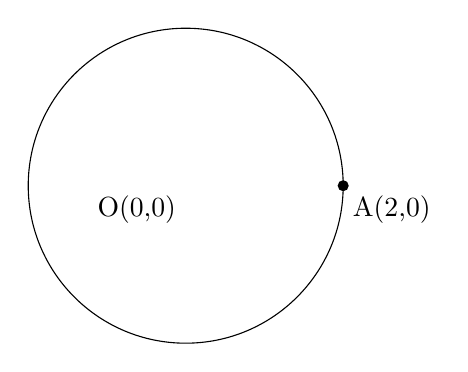
\begin{tikzpicture}
    % 绘制圆
    \draw (0,0) circle (2cm);
    % 绘制圆心标注
    \node at (0,0) [below left] {O(0,0)};
    % 绘制一个点
    \fill (2,0) circle (2pt);
    \node at (2,0) [below right] {A(2,0)};
\end{tikzpicture}
\end{minted}

结果是标注了圆心O和点A的坐标:
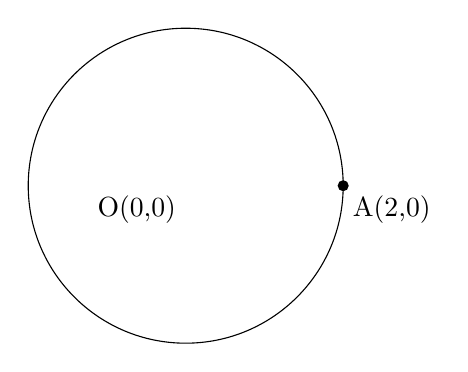
\begin{tikzpicture}
    % 绘制圆
    \draw (0,0) circle (2cm);
    % 绘制圆心标注
    \node at (0,0) [below left] {O(0,0)};
    % 绘制一个点
    \fill (2,0) circle (2pt);
    \node at (2,0) [below right] {A(2,0)};
\end{tikzpicture}
\end{block}
\end{frame}

\end{document}
